\section{Experimentos y Discusi\'on}
\subsection{Desv\'ios}

En este experimento realizamos un an\'alisis sobre los desv\'ios de los vuelos en base al tiempo. Dividimos al año en 12 meses y tomamos el per\'iodo 2000-2008. Para generar un an\'alisis representativo del comportamiento a escala pa\'is decidimos tomar 2 estados con caracter\'isticas particulares: deben tener gran cantidad de vuelos de llegada y deb\'ia ser uno de cada costa. De este modo tomamos a los estados de California y Florida para realizar el an\'alisis.

\subsubsection{California}

En el siguiente gr\'afico se puede observar el porcentaje de vuelos desviados en el per\'iodo mencionado para vuelos con destino a California.

\begin{figure}[h!]
  \begin{center}
	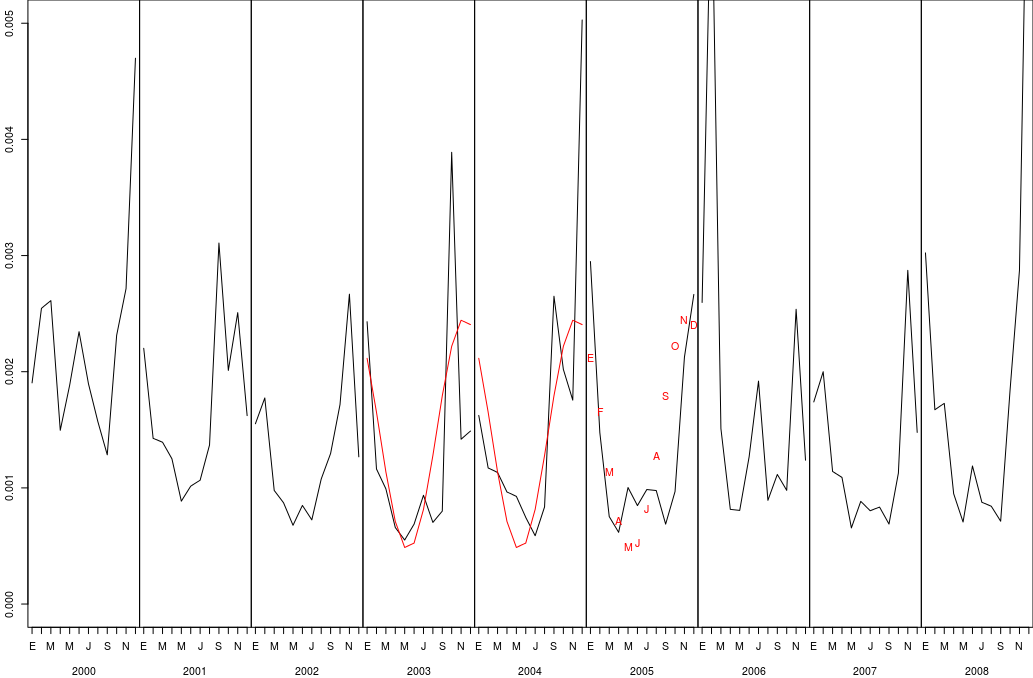
\includegraphics[scale=0.4]{img/plot_CA_2003-2005.png}
	\caption{Diverted arrivals - California}
  \end{center}
\end{figure}

Para aproximar a la funci\'on observamos algunas cosas:
\begin{itemize}  
\item Hay cierta periodicidad en la funci\'on. Posee picos en los meses correspondientes a las vacaciones de verano del hemisferio norte y descensos en el resto. El per\'iodo es de 12 meses.
\item Aunque la funci\'on tiene picos marcados, su forma se asemeja a la de $sin$ y $cos$.
\end{itemize}

Dados estos indicios nos proponemos encontrar una familia de funciones para aproximar nuestro gr\'afico usando cuadrados m\'inimos. Estas funciones ser\'an una combinaci\'on de $sin$ y $cos$ con per\'iodo 12. Las siguientes 2 familias de funciones responden a estas caracter\'isticas y aproximan relativamente bien a nuestra funci\'on, dados $alpha_i$ correspondientes.


$F_1 = \alpha_1 * abs(sin(\frac{\pi}{12}*x) * cos(\frac{\pi}{6}*x)^2) + \alpha_2$

$F_2 = \alpha_1 * sin(\frac{\pi}{6}*x) + \alpha_2 * cos(\frac{\pi}{6}*x) + \alpha_3$


La primera multiplica al $sin$ y $cos$ y toma el valor absoluto para eliminar los picos negativos. La segunda realiza la suma de los $sin$ y $cos$. No es relevante ac\'a tomar el valor absoluto ya que no hay picos marcados negativos. Luego a ambas funciones le sumamos una constante para que la curva se desplace en direcci\'on vertical. Observamos que sumar una variable lineal no ten\'ia impacto apreciable en la aproximaci\'on. 

Luego resolvimos cuadrados m\'inimos para ambas funciones y calculamos el error cuadr\'atico medio de cada una. Como training tomamos a los años 2003 y 2004 e intentamos predecir 2005.

Los errores cuadr\'aticos medios son: $ECM(F_1) = 0.0003236866$ y $ECM(F_2) = 0.0002451076$, siendo la segunda funci\'on una mejor aproximaci\'on que la primera. Los valores son pequeños ya que las mediciones son sobre un porcentaje pequeño.

Por lo tanto se puede ver en el gr\'afico anterior la aproximaci\'on que $F_2$ realiza en la muestra, prediciendo c\'omo ser\'a 2005. Se ve que respeta el comportamiento general y aproxima el pico que hay a principio y fin de año.

\subsubsection{Florida}

Realizamos el mismo an\'alisis para los vuelos dirigidos a Florida. La funci\'on sigue teniendo un comportamiento peri\'odico a\~no a a\~no, pero, como se puede apreciar en \ref{diverted-arrivals-florida}, vemos que por alg\'un motivo hay un desplazamiento horizontal de la curva: los picos positivos se encuentran a mitad de a\~no.
Por otro lado, el porcentaje de vuelos desviados est\'a en el mismo rango que en California.
Dado este conjunto de similitudes y diferencias con el caso anterior, nos interes\'o ver c\'omo se comportaban nuestras familias de funciones anteriores para aproximar a nuestra nueva curva.

Para esto realizamos cuadrados m\'inimos con las siguientes dos familias de funciones:

$F_1 = \alpha_1 * abs(sin(\frac{\pi}{12}*x) * cos(\frac{\pi}{6}*x)^2) + \alpha_2$

$F_2 = \alpha_1 * sin(\frac{\pi}{6}*x) + \alpha_2 * cos(\frac{\pi}{6}*x) + \alpha_3$

y vimos que los errores cuadr\'aticos medios en este caso fueron de $ECM(F_1) = 0.0003098236$ y $ECM(F_2) = 0.0003590168$, o sea, bastante similares al anterior.

Se puede observar la curva en el siguiente gr\'afico:

\begin{figure}[h!]
  \begin{center}
	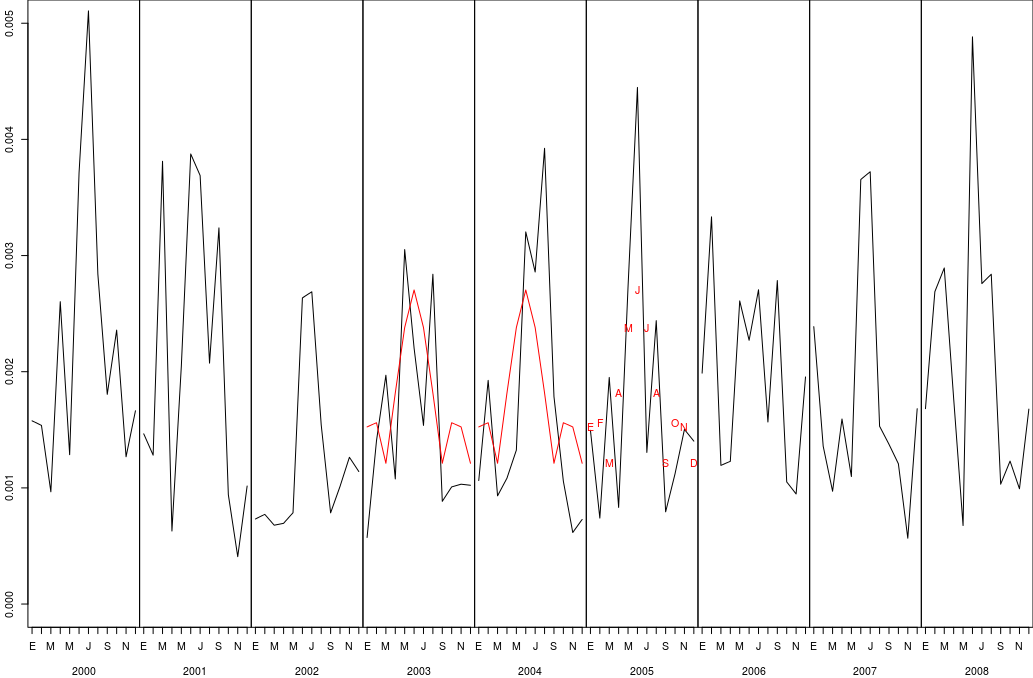
\includegraphics[scale=0.4]{img/plot_FL_2003-2005.png}
	\caption{Diverted arrivals - Florida}
  \end{center}
  \label{diverted-arrivals-florida}
\end{figure}

Una raz\'on que puede ser atribu\'ida a este fen\'omeno es el hecho de que la temporada de huracanes coincide con los meses donde se presentan los picos (el verano del hemisferio norte). Con lo cu\'al, tiene sentido que se presente un mayor porcentaje de desv\'ios para sortear estas condiciones clim\'aticas adversas. Quisimos crear una familia de funciones parecida a las que ten\'iamos pero que considerase esa particularidad.
Probando un poco nos dimos cuenta que las potencias de $cos$ tienen un comportamiento de este estilo. Por ejemplo $5*cos(x)^{500} + 1$ tiene el siguiente gr\'afico:

\begin{figure}[h!]
  \begin{center}
	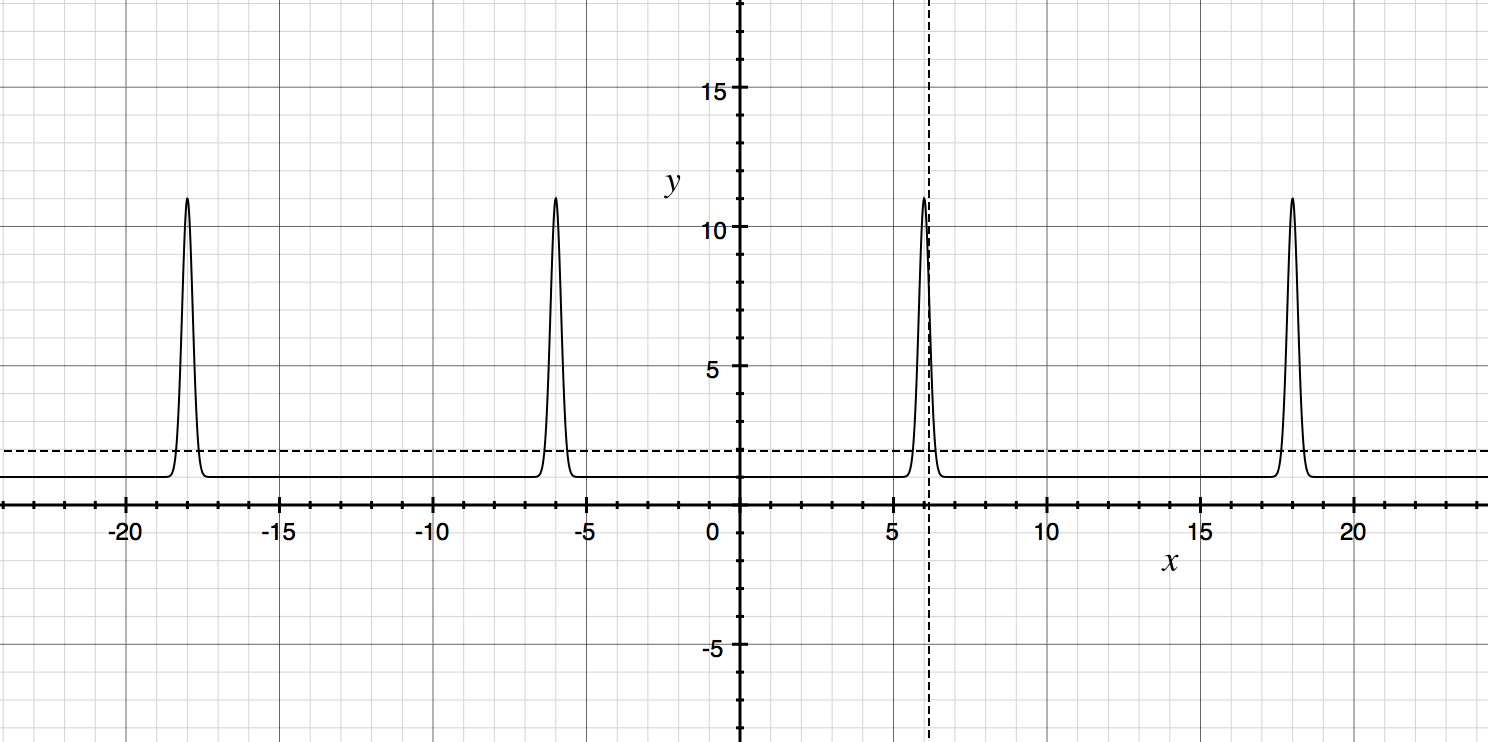
\includegraphics[scale=0.4]{img/cos500.png}
	\caption{$5*cos(x)^{500} + 1$}
  \end{center}
\end{figure}

Por lo tanto llegamos a la siguiente familia de funciones que usa esta nueva t\'ecnica.

$F_3 = \alpha_1 * abs(sin(\frac{\pi}{12}*x) * cos(\frac{\pi}{6}*x)^2) + \alpha_2 * cos(\frac{\pi}{12}*x - \frac{\pi}{2})^{500} + \alpha_3$

El error cuadr\'atico medio de esta funci\'on es $ECM(F_3) = 0.00030524$.

Podemos ver a $F_3$ representada en el gr\'afico de Florida en rojo. En ese caso se entren\'o cuadrados m\'inimos con 2003 y 2004 y se predice 2005.

\subsection{Desv\'ios por distancia}

Otro eje de análisis que nos pareció interesante fue investigar qué ocurría con la cantidad de vuelos que se desvían en relación a la distancia del viaje. Este eje surge de la idea de que a mayor distancia del viaje, mayor probabilidad de que surjan problemas en el trayecto, ya sean desperfectos técnicos, mal clima o situaciones impredecibles.

Para esto realizamos el siguiente gráfico que muestra el porcentaje de vuelos desviados según la distancia del vuelo. Como los vuelos tienen hasta 5 mil millas de distancia, partimos a nuestro conjunto en 10 subconjuntos (0 a 500 millas, 501 a 1000 millas, ..., 4501 a 5000 millas).

\begin{figure}[h!]
  \begin{center}
	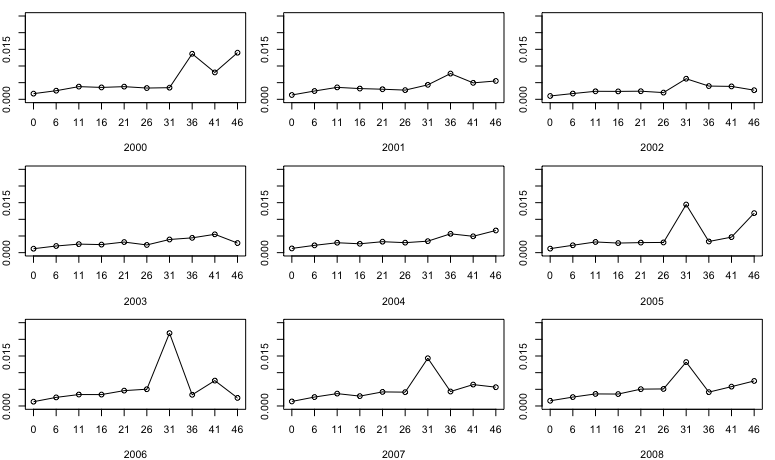
\includegraphics[scale=0.5]{img/diverted_by_distance.png}
	\caption{Diverted by distance}
  \end{center}
\end{figure}

Hay algunas cosas que se pueden ver rápidamente en el gráfico. 
Por un lado vemos que año a año la curva respeta cierto patrón. 
Por otro lado se puede ver que el gráfico acompaña la hipótesis del aumento de desvíos según la distancia del vuelo, a pesar de que la pendiente es casi nula.
La más llamativa de las características del gráfico es que en el segmento de 3001 a 3500 millas hay un pico muy llamativo, donde la cantidad de vuelos desviados llega a triplicar su valor en los segmentos aledaños. Lo más extraño es que aunque pareciera ser un outlier, este evento se da año a año, en particular entre 2005 y 2008.

Nos propusimos analizar esta situación para esclarecer sus causas. Para eso tomamos como referencia el año 2006. Primero calculamos la cantidad de vuelos que hay para cada segmento y vimos que decrece exponencialmente: mientras que para vuelos de menos de 500 millas hubo más de 3 millones, a partir de 3 mil millas los segmentos tienen menos de 5 mil vuelos. Por lo tanto los outliers tienen mucho más peso. Luego quisimos averiguar qué aeropuertos eran los que más desvíos tuvieron en el segmento del pico y los resultados son llamativos: de 47 vuelos desviados, 43 pertenecen a 2 vuelos en particular, los que vuelan entre DEN y HNL, y los que vuelan entre IAH y ANC.
Por lo tanto este pico se debe exclusivamente a características de estos 2 vuelos. Puede ser un tema climático de la ruta que utilizan, o de la administración interna de los aeropuertos con esos vuelos. Sea cual sea el motivo, es responsabilidad de muy pocos y se manifiesta en el gráfico de ese modo debido a la poca cantidad de vuelos de tanta distancia.



